\documentclass[a4paper, fontsize=12pt, ngerman, oneside, openright]{scrreprt}

% Rendering packages
\usepackage{amsmath}
\usepackage{amssymb}
%\usepackage[draft]{graphicx}
\usepackage{graphicx}
\usepackage{wrapfig}
\usepackage{svg}
\usepackage{subcaption}
\usepackage{placeins}
\usepackage{xcolor}      % use if color is used in text
\usepackage{eurosym}


% Page dimensions
\usepackage[inner=2.5cm,outer=2.5cm,top=3.7cm,bottom=3.5cm]{geometry} 
\usepackage{parskip}
\usepackage[onehalfspacing]{setspace}

% Font styling
\usepackage[english]{babel}
\usepackage[utf8]{inputenc}
\usepackage[T1]{fontenc}
\usepackage{lmodern}
\renewcommand\familydefault{\sfdefault}
\usepackage[11pt]{moresize}

% Tables
\usepackage{tabularx}
\usepackage{tabulary}
\usepackage{longtable, lscape}

% Headers
\usepackage{scrpage2}  % header and footer for KOMA-Script
\pagestyle{scrheadings}
\automark[section]{chapter}

% Zitate
\usepackage[backend=biber, 
			style=authoryear,
			isbn=false, 
			sorting=nyt,
			]{biblatex}
\usepackage[babel,german=quotes, english=british, threshold=3]{csquotes}
\bibliography{Bibliothek/Bibliothek}

\usepackage[hyperindex,breaklinks,colorlinks=true,linkcolor=black,urlcolor=blue,citecolor=black]{hyperref}

% Code Blöcke
\usepackage{listings}
%\usepackage{Header/listings-golang} % import this package after listings
\usepackage{syntax}



%\lstset{ % add your own preferences
%	frame=single,
%	captionpos=b,
%	mathescape=true,
%	basicstyle=\footnotesize\ttfamily,
%	keywordstyle=\color{black},
%	numbers=left,
%	numbersep=5pt,
%	showstringspaces=false, 
%	stringstyle=\color{blue},
%	tabsize=2,
%	language=Golang % this is it !
%}


%table colors
\usepackage{xcolor,colortbl}

\newcommand{\mc}[2]{\multicolumn{#1}{c}{#2}}
\definecolor{Gray}{gray}{0.85}
\definecolor{LightCyan}{rgb}{0.88,1,1}

\newcolumntype{a}{>{\columncolor{Gray}}c}
\newcolumntype{b}{>{\columncolor{Gray}}l}

\usepackage{color}
\definecolor{gray}{rgb}{0.4,0.4,0.4}
\definecolor{darkblue}{rgb}{0.0,0.0,0.6}
\definecolor{cyan}{rgb}{0.0,0.6,0.6}
\definecolor{dkgreen}{rgb}{0,0.6,0}
\definecolor{gray}{rgb}{0.5,0.5,0.5}
\definecolor{mauve}{rgb}{0.58,0,0.82}

\lstset{
  basicstyle=\ttfamily,
  columns=fullflexible,
  showstringspaces=false,
  commentstyle=\color{gray}\upshape
}

\lstset{
	frame=tb,
	language=Java,
	aboveskip=3mm,
	belowskip=3mm,
	showstringspaces=false,
	columns=flexible,
	basicstyle={\small\ttfamily},
	numbers=none,
	numberstyle=\tiny\color{gray},
	keywordstyle=\color{blue},
	commentstyle=\color{dkgreen},
	stringstyle=\color{mauve},
	breaklines=true,
	breakatwhitespace=true,
	tabsize=3,
	numbers=left
}

\lstdefinelanguage{XML}
{
	morestring=[b]",
	morestring=[s]{>}{<},
	morecomment=[s]{<?}{?>},
	morecomment=[s]{!--}{--},
	stringstyle=\color{black},
	identifierstyle=\color{darkblue},
	keywordstyle=\color{cyan} list your attributes here
}

%pdf insert
\usepackage{pdfpages}

%zusätzliche Trennungen
\hyphenation{Grund-ar-chi-tek-tur}
\hyphenation{MQTT-Kom-mu-ni-ka-tions-mo-dell}
\hyphenation{Master-Master-Replikation}
\hyphenation{Pub-lish-er}
\hyphenation{Pub-lish-ers}
\hyphenation{Sub-scriber}
\hyphenation{Sub-scribers}
\hyphenation{Pub-lish er/Sub-scriber}
\hyphenation{beo-bacht-bar}
\hyphenation{Score}
\hyphenation{Ac-knowl-edge-ment}
\hyphenation{Ac-knowl-edge-ments}

\usepackage{mathtools}
\DeclarePairedDelimiter\abs{\lvert}{\rvert}

\usepackage{acronym}



\begin{document}

% Titelseite einfügen.
\begin{titlepage}


\begin{center}
 		
\includegraphics[scale=0.3]{Resources/Logo3}
\end{center}

\begin{center}
	\HUGE \textbf{Varroa}
	\large\\MQTT-Scenario-Testing-Tool\\ \ \\
	\small Masters Level Study Project, Prof. PhD. Siebert \\
	SS 2018 - WS 2018/2019
\end{center}

\begin{center}
R. Atherton, S. Baier, S. Giebl, G. Held, Y. Weber, T. Weiden
\end{center}

\end{titlepage}


\clearpage

% Counter zurücksetzen. Römische Ziffern einstellen.
\pagenumbering{Roman}
\setcounter{page}{1}

% Inhaltsverzeichnis generieren.
\tableofcontents

% Neue Seite. Counter zurücksetzen. Arabische Ziffern einstellen.
\clearpage
\pagenumbering{arabic}
\setcounter{page}{1}

% Kapitel einfügen.
\chapter{Vision}
The motivation for creating \emph{Varroa} -- a MQTT testing tool -- was the lack of testability of MQTT systems.
The name \emph{Varroa} is inspired by the varroa mite, which is a species of mite that infects honey bee colonies.
Figuratively our MQTT testing tool works in a similar way but instead of infesting a hive, it tries to infest a broker.
This association between the bee hives of the natural realm and those of the MQTT world came from the \emph{HiveMQ} MQTT broker's branding.


The basic use-case of \emph{Varroa} is testing the resilience of brokers by creating load.
To achieve this, \emph{Varroa} is able to simulate a large amount of MQTT clients by a simple and descriptive Scenario definition.
A Scenario can be easily declared by a domain specific language which is defined in a XSD file.


Furthermore Varroa can be executed as a distributed system.
If this is the case the workload is automatically split and distributed to different machines.
This enables great horizontal scaling potential.
In this context scaling means that the amount of MQTT clients can easily be increased.



\chapter{Concepts}
To understand the workings of Varroa, we will have to take a look at the different parts that make up the system.
Furthermore we explain the basic concepts of MQTT.

\section{Varroa Distributed System Concepts}
A Varroa Distributed System is an orchestration of multiple Varroa Instances consisting of one Commander and at least one Agent.
Varroa is organized as a distributed system due to the impossibility of creating enough MQTT clients on a single machine to overload an MQTT broker, especially if the broker is also a distributed system.

\paragraph{Varroa Instance}
A Varroa instance is a running Varroa process in a single JVM, which can be a Commander and/or an Agent.

\paragraph{Commander}
The Commander is a part of the Varroa Distributed system that processes the Scenario.
It distributes the workload of the Scenario to the Agents through Chunks.
Only one Commander exists in a Varroa Distributed System.

\paragraph{Agent}
Agents are part of the Varroa Distributed System.
They are responsible for executing the Scenarios workload by receiving Chunks from the Commander and passing them to their MQTT Agents.
A Varroa Distributed System contains at least one Agent.

\paragraph{MQTT Agent}
MQTT Agents are components of an Agent.
Every MQTT Agent manages one MQTT client.

\paragraph{Chunk}
The Scenario is split in Chunks by the Commander and then those Chunks are distributed to the Agents.

\section{Varroa Scenario Concepts}
The integral idea of Varroa is testing Scenarios, which means simulating the behaviour of a large amount of MQTT clients.
It tests whether the MQTT broker can handle the load associated with these clients.
A Scenario is an abstract representation of a real MQTT use case.
It defines the topology of all participating MQTT clients and brokers.

\paragraph{Client Group}
Client Groups are a part of the Scenario.
They enable the user to define an abstract group of MQTT clients with similar behaviour and properties.

\paragraph{Topic Group}
A Topic Group represents a number of topics that share a naming pattern.
This concept enables the user to model the interaction between Client Groups and a number of similar topics.

\paragraph{Stage}
Stages are execution steps of the Scenario. Stages are executed serially.

\paragraph{Lifecycle}
Lifecycles are part of a Stage.
One Lifecycle defines the behaviour of one Client Group within the Stage.
The Lifecycles contained in a Stage are executed in parallel.

\paragraph{Command}
A Lifecycle consists of multiple Commands.
A Command is an abstract representation of a work step that must be executed by a MQTT Agent.

\paragraph{Action}
An Action is an actual execution of a Command by a MQTT Agent.

\section{General MQTT Concepts}

\paragraph{MQTT Broker}
The broker serves as an intermediary between publishers and subscribers.
It takes over the routing of the exchanged MQTT messages and is the central control authority of a MQTT network.
%TODO cite Georg

\paragraph{MQTT Client}
A client that implements the MQTT protocol.
We use the \emph{HiveMQ MQTT Client} as an implementation.

\paragraph{Topic}
Topics are strings separated by slashes that do not contain wildcards.
Messages published with a topic are delivered to subscribers that have registered matching Topic Filters.

\paragraph{Topic Filter}
A Topic Filter is a chain of strings delimited by slashes that 
can cover one or more topics. 
It can also contain wildcards: a single plus character covers one hierarchy level, a double cross selects all possible following levels.

\paragraph{Publish}
Publishers are clients that produce data.
They send messages with a specific Topic to the broker.

\paragraph{Subscribe}
Subscribers are clients that subscribe to a subset or to all messages sent via the
MQTT network.
They log on to the broker and register with one or more Topic Filters that specify the topics, which determine what messages they want to receive.
%TODO cite Georg




\chapter{Architecture}\label{sec:Architecture}
Varroas architecture is organised as a distributed system, whereas there are two main roles in the system: the Agents and the Commander.
The Commander is the central unit that passes work packages of the Scenario to the Agents.
In contrast the Agents process the passed packages and create MQTT clients to execute them.
%The Commander parses the Scenario, splits it into chunks and then distributes it among the agents.

\section{Varroa Distributed System Architecture}
\begin{figure}[h]
	\begin{center}
	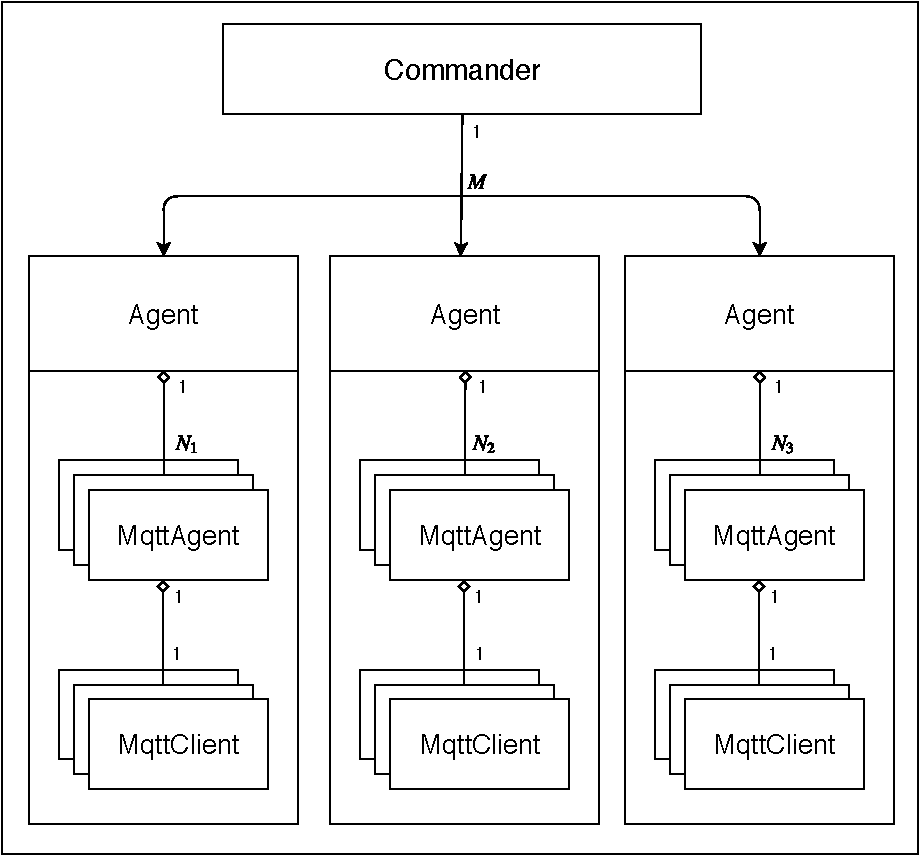
\includegraphics[scale=0.65]{Resources/PDF/Architecture}
	\caption{Varroa Distributed System Architecture}
	\label{pic:Architecture}
	\end{center}
\end{figure}
A Varroa Distributed System is composed of a Commander and multiple Agents.
The Commander and all Agents are executed in separate Varroa Instances.
Every Agent holds a number of MQTT Agents and each MQTT Agent manages one MQTT Client.
\newpage

\section{Chunk Concept}
A chunk is a work package of the scenario execution designed to be distributed from the Commander to its Agents.
It is then handled by the Agent it is distributed to.
The Agent then creates or uses existing MQTT Agents to execute the Chunk.
The most important contained bits of information are:
\begin{itemize}
	\item \textbf{clientGroupId}: identifier for the Client Group the Chunk should be executed for.
	\item \textbf{clientGroupInformation}: contains information concerning the Client Group.
	\item \textbf{clientCountInChunk}: the amount of clients the Chunk represents.
	\item \textbf{clientOffset}: starting index of the clients inside the Client Group. clientOffset and clientCountInChunk identify the subset of clients out of the Client Group this Chunk is executed for.
	\item \textbf{actionOffset}: identifies the index of the first action that should be executed -- acts like a program counter in the Scenario.
	\item \textbf{commands}: a list of commands that are executed by the clients in the Chunk.
\end{itemize}

\section{Chunk Distribution}\label{sec:chunkDistribution}
\begin{figure}[h]
	\begin{center}
	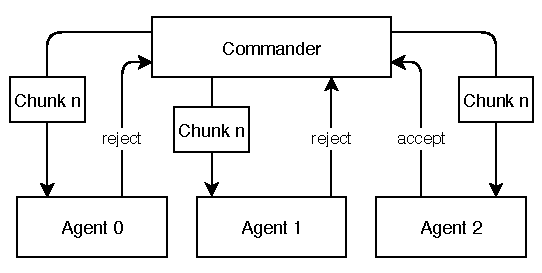
\includegraphics[scale=1.2]{Resources/PDF/ChunkDistribution}
	\caption{Distribution of a Chunk}
	\label{pic:ChunkDistribution}
	\end{center}
\end{figure}
A Chunk is deterministically assigned to an Agent to ensure that it gets executed by the same Agent even on multiple runs of the scenario. This determinism is needed to avoid fluctuation of reporting results that would be caused by Varroa and not the MQTT system under test.
To ensure this determinism a round-robin distribution of the scenario's Chunks combined with a handshake mechanism is used:
In accordance to figure \ref{pic:ChunkDistribution} the Commander tries to distribute a Chunk to an Agent who then answers with an accept or reject.
If the Agent rejects the Chunk (see figure \ref{pic:RejectHandshake}) the Commander then tries to distribute the Chunk to the next Agent in the same manner until one Agent accepts.
When accepting the Chunk the Agent waits for a start message from the Commander and upon receiving it the Agent starts executing the Chunk.
After a successful execution of the Chunk the Agents sends a finished message to the Commander (see figure \ref{pic:AcceptHandshake}).


\begin{minipage}[ht]{0.48\textwidth}
	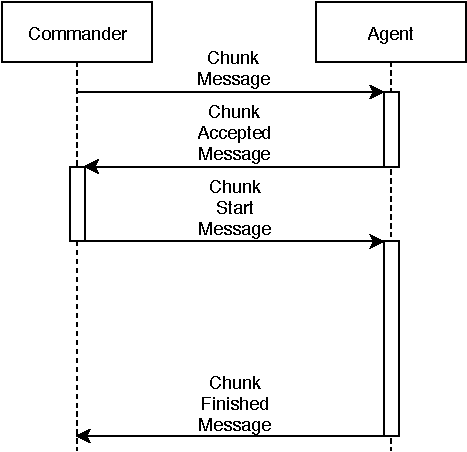
\includegraphics[width=\textwidth]{Resources/PDF/ChunkAcceptedHandshake}
\end{minipage}
\hfill
\begin{minipage}[ht]{0.48\textwidth}
	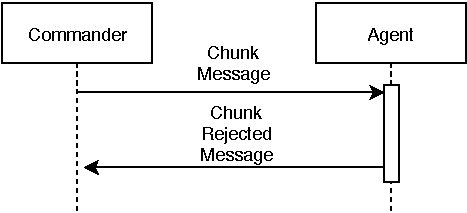
\includegraphics[width=\textwidth]{Resources/PDF/ChunkRejectHandshake}
\end{minipage}

\begin{minipage}[ht]{0.48\textwidth}
	\captionof{figure}{Chunk Handshake with Accept}
	\label{pic:AcceptHandshake}
\end{minipage}
\hfill
\begin{minipage}[ht]{0.48\textwidth}
	\captionof{figure}{Chunk Handshake with Reject}
	\label{pic:RejectHandshake}
\end{minipage}

\chapter{Execution}\label{sec:Execution}
To start a Varroa test the user needs to start a Commander and at least one Agent.
The Agents periodically tries to establish a connection to the Commander.
Once all Agents are connected the execution of the scenario starts.\\

\section{Commander}
\begin{figure}[H]
	\begin{center}
	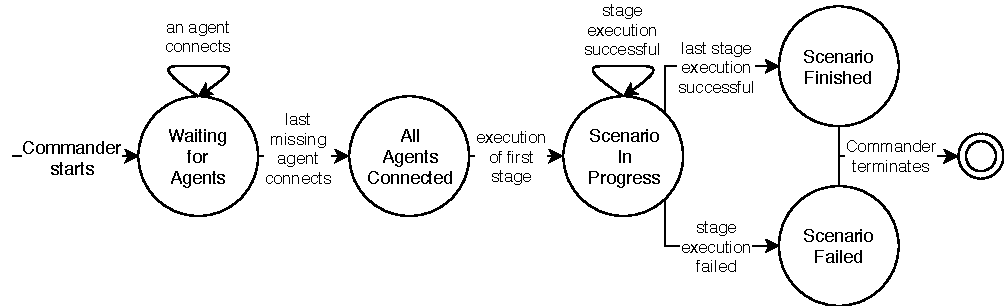
\includegraphics[scale=0.9]{Resources/PDF/CommanderStates}
	\caption{Commander States}
	\label{pic:CommanderStates}
	\end{center}
\end{figure}
When starting a Varroa Instance that is configured as a Commander (see \ref{sec:commanderConfig}) it performs the following actions:
\begin{itemize}
	\item First it parses and validates the Scenario.
	\item Then it waits for the Agents to connect.
	Until all Agents are successfully connected it remains in the \emph{Waiting for Agents} state.
	As the last missing Agent has connected to the Commander it switches its state to \emph{All Agents Connected}.
	\item When all Agents are connected, the Commander starts to distribute the Scenario data amongst the Agents. After this is finished the state is set to \emph{Scenario Data Distributed}.
	\item After the preceding initiation steps the actual distribution and execution of the Scenario is started.
	In doing so the Commander changes its state to \emph{Scenario in Progress}.
	In this state it distributes the Stages of the Scenario one after each other to the Agents.
	It remains in this state until all Stages are successfully executed and then transfers its state into \emph{Scenario Finished}.
	If one execution of a Stage errors this results in the failure of the whole Scenario -- logically the Commanders state is then \emph{Scenario Failed}.
	\item As the last step the Commander always -- independent of execution success -- generates the final Report by aggregating the partial reports from the Agents.
\end{itemize}

To allow better comprehension \figurename{} \ref{pic:CommanderStates} illustrates this process.

\section{Agent}
\begin{figure}[H]
	\begin{center}
	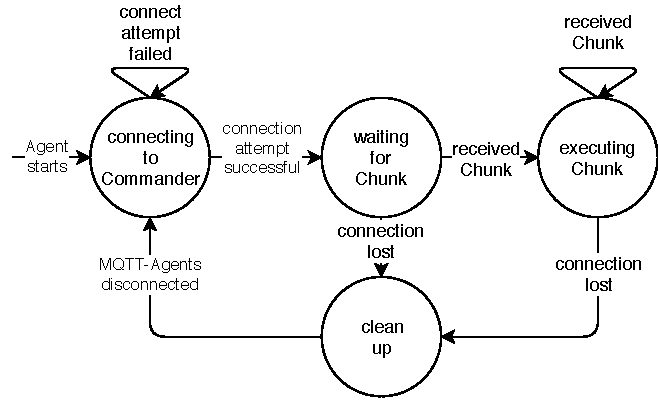
\includegraphics[scale=0.9]{Resources/PDF/AgentStates}
	\caption{Agent States}
	\label{pic:AgentStates}
	\end{center}
\end{figure}
Upon starting a Varroa Instance as an Agent (see \ref{sec:agentConfig}) it performs the following actions:
\begin{itemize}
	\item First it tries to connect to the configured Commander.
	It periodically attempts to establish the connection until it succeeds.
	\item Then it waits for incoming Chunks from the Commander and executes them, implementing the handshake protocol that will be introduced in \ref{sec:chunkDistribution}.
	The Agent continues doing so until the Connection is closed by the Commander, which means the Scenario is executed completely.
	\item In contrast to the Commander the Agent process does not terminate after the execution of a Scenario. Instead it returns to the first step and tries to reconnect to a Commander.
	Because of this the user only needs to restart the Commander to execute another Scenario.
\end{itemize}

For better understanding of the temporal processes the just explained concepts are illustrated in figure \ref{pic:AgentStates}.

\section{Configuration}
Varroa can be run with two different ways of configuration.
One is to configure Varroa ahead of time -- manually or programmatically.
The other is to use containers and utilize dynamic discovery of the Varroa Instances.

\subsection{Static configuration}
\begin{figure}[h]
\begin{center}
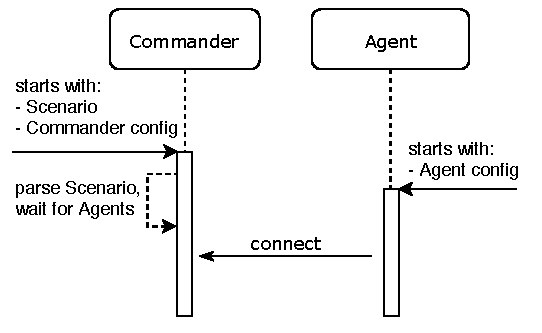
\includegraphics[scale=1]{Resources/PDF/ExecutionStaticInit}
\caption{Static configuration}
\label{pic:staticExecution}
\end{center}
\end{figure}

A static configuration may be used on any infrastructure where the hostnames or IP addresses of all Varroa Instances (Commander and Agents) are known ahead of time. This is the case on most of the typically used systems, such as IaaS clouds where an instance is booted and is assigned an address before the application is deployed onto the system.\\
\\
To configure Varroa statically the user must provide an Instance configuration, which sets up the Varroa Instance as a Commander or an Agent.
It is also possible to configure a single Varroa Instance as both Commander and Agent.
This allows simple execution of small tests on a single machine.
\\
If the Varroa Instance is configured as a Commander the user must also provide a Scenario.
\\
Both Instance configuration and the Scenario are defined in XML files.
These are referenced by the command line parameters -I and -S:
\begin{lstlisting}[caption={Command line configuration examples}, captionpos=b, label={lst:commanderConfig}, language=bash]
java -jar varroa-1.0.jar -I path/to/commander.xml -S path/to/scenario.xml
java -jar varroa-1.0.jar -I path/to/agent.xml
\end{lstlisting}

A detailed description of the Instance configuration options can be found below.

\subsubsection{Commander configuration}\label{sec:commanderConfig}
\begin{lstlisting}[caption={Commander XML configuration example}, captionpos=b, label={lst:commanderConfig}, language=XML]
<varroa>
    <commander>
		<bind-host>192.127.0.1</bind-host>
        <bind-port>12345</bind-port>
        <amount-agents>3</amount-agents>
    </commander>
</varroa>
\end{lstlisting}
\begin{itemize}
	\item \textbf{bind-host:} specifies the address the Commander will accept Agent connections on.
	\item \textbf{bind-port:} specifies the port the Commander waits for Agent connections on.
	\item \textbf{amount-agents:} specifies the amount of Agents that the Commander awaits.
\end{itemize}

\subsubsection{Agent configuration}\label{sec:agentConfig}
\begin{lstlisting}[caption={Agent XML configuration example}, captionpos=b, label={lst:agentConfig}, language=XML]
<varroa>
    <agent>
		<commander-host>192.127.0.1</commander-host>
        <commander-port>12345</commander-port>
        <local-port>23458</local-port>
		<commander-retry-interval>10</commander-retry-interval>
    </agent>
</varroa>
\end{lstlisting}
\begin{itemize}
	\item \textbf{commander-host:} specifies the address of the Commander to connect to.
	\item \textbf{commander-port:} specifies the port of the Commander.
	\item \textbf{local-port:} specifies the local port the Agent uses for the outgoing connection to the Commander.
	\item \textbf{commander-retry-interval:} the time interval in seconds in which the Agent tries to connect to the Commander.
\end{itemize}

\subsection{Dynamic configuration}

\begin{figure}[h]
\begin{center}
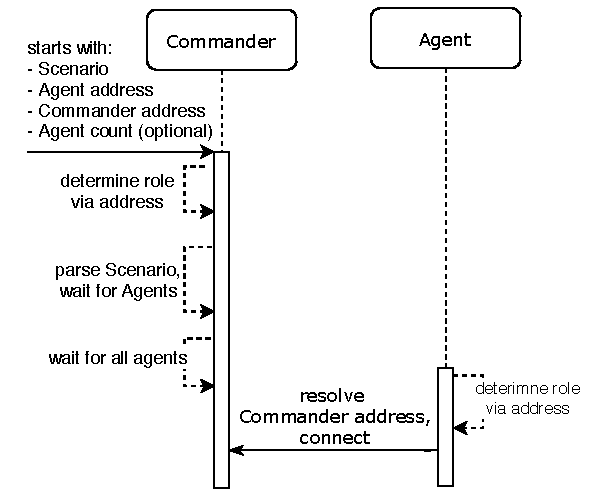
\includegraphics[scale=1]{Resources/PDF/ExecutionDnsInit}
\caption{dynamic execution}
\label{pic:dynamicExecution}
\end{center}
\end{figure}

DNS discovery is specifically aimed at container environments and cloud platforms. These types of platforms generally provide different methods of service discovery, which are necessary to allow the parts of a distributed system to communicate with each other.

In container environments, the address of a server where an application is going to run on is generally not known ahead of application startup. Containers are launched quickly and in an unpredictable order, leading to a scenario where the addresses of all parts of a system are unknown ahead of time. This necessitates a configuration method which allows service discovery after application startup, which the previous method cannot handle.


Dynamic configuration allows Varroa to start without knowing the addresses of any other Varroa instances nor its own role. The way the initial DNS discovery method works is by supplying hostnames for the Commander and Agent groups respectively.


\begin{figure}[h]
\begin{center}
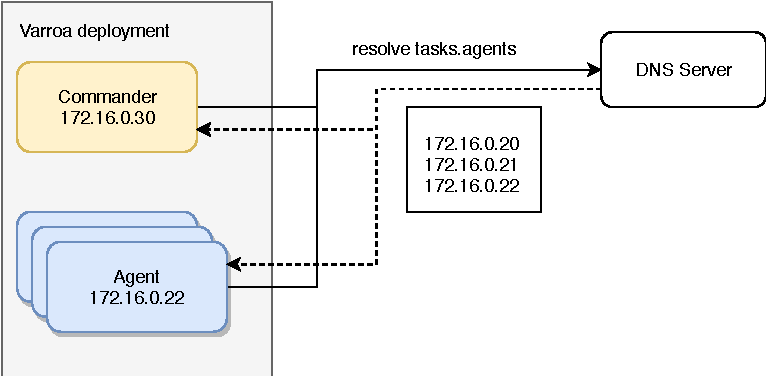
\includegraphics[scale=0.8]{Resources/PDF/ExecutionDnsDiscovery}
\caption{agent record resolution}
\end{center}
\end{figure}

During start up Varroa will continuously resolve these records, which must be designed as round-robins.
Then each address found in the records is compared to the address corresponding to its own hostname. 
If a match is found, the instance will set its role according to the set of addresses it matches.

Additionally, Agents can use the commander address to locate the commander node and continuously attempt to connect to it until it is ready for Agent connections.

The commander can also determine how many Agents will connect to it using the Agent address, or alternatively a Agent count can be  provided at startup (for deployments on services where records are slowly updated as containers start).

\begin{figure}[h]
\begin{lstlisting}
VARROA_DNS_AGENT=tasks.agents
VARROA_DNS_COMMANDER=tasks.commander
VARROA_DNS_AGENT_COUNT=3
\end{lstlisting}
\caption{A sample dynamic discovery configuration, showing the environment variable values}
\end{figure}

\chapter{Scenario Concept}\label{sec:ScenarioConcept}
\setlength{\grammarparsep}{20pt plus 1pt minus 1pt} % increase separation between rules
\setlength{\grammarindent}{12em} % increase separation between LHS/RHS 
%\begin{lstlisting}[caption={Implementierung des Trainierens der Markov-Chain}, captionpos=b, label={lst:train}, language=XML]
% <!-- -->
%\end{lstlisting}

A Varroa test is the execution of a user defined Scenario, which is specified in a XML file.
To define a valid scenario the user needs to define the topology of the Scenario and the behaviour of its components.

For the description of a scenario Varroa uses a small Domain Specific Language, which is realized in XML and adheres to the following grammar:
\begin{grammar}
	<scenario> := 				<descriptors><stages>
	
	<descriptors> :=			<requiredDescriptors><optionalDescriptors>
	
	<requiredDescriptors> := 	<broker><clientGroups><topicGroups>
	
	<optionalDescriptors> := 	<subscriptions><waitPatterns>
								\alt <subscriptions>
								\alt <waitPatterns>
								\alt <empty>
\end{grammar}

More exact definition of the productions will be given further along this chapter. As the default implementation of the Varroa DSL is in XML most productions start with a opening XML tag and end with a closing XML tag. For brevity these are not explicitly described in the grammar.

An example for the outline of a Scenario XML file is given in \ref{lst:scenario}.

\begin{lstlisting}[caption={example for the XML definition of the Scenario}, captionpos=b, label={lst:scenario}, language=XML]
<scenario>
	<broker id="b1">
		<!-- definition broker parameters -->
	</broker>
	
	<clientGroups>
		<!-- definition of client groups -->
	</clientGroups>
	
	<topicGroups>
		<!-- definition of topic groups -->
	</topicGroups>
	
	<subscriptions>
		<!-- definition of subscriptions -->
	</subscriptions>

	<waitPatterns>
		<!-- definition of waitPatterns -->
	</waitPatterns>
	
	<stages>
		<!-- definition of stages -->
	</stages>
</scenario>
\end{lstlisting}

\section{Broker}

\begin{grammar}
	<broker> := <brokerAttributes>
\end{grammar}

\begin{lstlisting}[caption={example for the XML definition of the Broker}, captionpos=b, label={lst:broker}, language=XML]
<scenario>
	<broker id="b1">
		<address>broker.hivemq.com</address>
		<port>1883</port>
	</broker>
</broker>
\end{lstlisting}
The broker is the central component whose performance and stress resistance is tested by the Scenario.
For this the user needs to define:
\begin{itemize}
	\item \textbf{id:} the identifier to reference the broker.
	\item \textbf{address:} the address of the broker can either be a IPv4-Address or a Fully-Qualified-Domain-Name.
	\item \textbf{port:} the port on which the broker is waiting for connections.
\end{itemize}

\section{Client Groups}

\begin{grammar}
	<clientGroups> := 	<clientGroup> <moreClientGroups>
						\alt <clientGroup>
						
	<moreClientGroups> := <clientGroup> <moreClientGroups>
							\alt <clientGroup>
	
	<clientGroup>  :=   <clientGroupAttributes>
\end{grammar}

\begin{lstlisting}[caption={example for the XML definition of Client Groups}, captionpos=b, label={lst:clientGroups}, language=XML]
<scenario>
	<clientGroups>
		<clientGroup id="cg1">
			<clientIdPattern>A[1-9]+</clientIdPattern>
			<count>100</count>
			<mqtt>
				<!-- MQTT properties -->
			</mqtt>
		</clientGroup>

		<!-- definition of more client groups -->
	</clientGroups>
</scenario>
\end{lstlisting}
A Scenario contains a number of Client Groups.
A Client Group is a specific amount of MQTT clients that share the exact same behaviour.
When defining a Client Group the user needs to specify:
\begin{itemize}
	\item \textbf{id:} the identifier to reference the Client Group.
	\item \textbf{clientIdPattern:} a regular expression to deterministically create individual names for every MQTT client in the Client Group.
	\item \textbf{count:} the amount of MQTT clients contained in the Client Group.
	\item \textbf{mqtt:} MQTT properties of the MQTT clients (see \lstlistingname{} \ref{lst:mqttProperties}).
	\begin{itemize}
		\item \textbf{version (requrired):} the MQTT version this Client Group implements.
		%TODO \item \textbf{cleanStart (optional):} 
		%TODO \item \textbf{sessionExpiryInterval (optional):}
	\end{itemize}
\end{itemize}

\begin{lstlisting}[caption={example for the XML definition of MQTT properties}, captionpos=b, label={lst:mqttProperties}, language=XML]
<mqtt>
	<version>5</version>
<\mqtt>
\end{lstlisting}
%	<cleanStart>true</cleanStart>
%	<sessionExpiryInterval>0x0</sessionExpiryInterval>
%</mqtt>	
%\end{lstlisting}


\section{Topic Groups} \label{sec:topicGroups}
\begin{grammar}
	<topicGroups> := 	<topicGroup><moreTopicGroups>
						\alt <topicGroup>
						
	<moreTopicGroups> := <topicGroup> <moreTopicGroups>
						\alt <topicGroup>
						
	<topicGroup>  :=    <topicGroupAttributes>
\end{grammar}
\begin{lstlisting}[caption={example for the XML definition of Topic Groups}, captionpos=b, label={lst:topicGroups}, language=XML]
<scenario>
	<topicGroups>
		<topicGroup id="tg1">
			<topicNamePattern>topic/subtopic-[0-9]{10}</topicNamePattern>
			<count>10</count>
		</topicGroup>

		<!-- definition of more topic groups -->
	</topicGroups>
</scenario>
\end{lstlisting}
A Scenario contains a number of Topic Groups.
A Topic Group is a specific amount of MQTT Topics whose names are created from the same regular expression.
When defining a Topic Group the user needs to specify:
\begin{itemize}
	\item \textbf{id:} the identifier to reference the Topic Group.
	\item \textbf{topicNamePattern:} a regular expression to deterministically create individual topic names for every member of the Topic Group.
	\item \textbf{count:} the amount of MQTT topics in the topic group.
\end{itemize}

\section{Subscriptions} \label{sec:subscriptions}
\begin{grammar}
	<subscriptions> :=		<subscription><moreSubscriptionsGroups>
							\alt <subscription>
	
	<moreSubscriptionsGroups> := 	<subscription> <moreSubscriptionsGroups>
							\alt <subscription>
	
	<subscription>  :=		<dynamicSubscription>
							\alt <topicFilter>
\end{grammar}
\begin{lstlisting}[caption={example for the XML definition of subscriptions}, captionpos=b, label={lst:subscriptions}, language=XML]
<scenario>
	<subscriptions>
		<subscription id="sub-1">
			<topicGroup>tg1</topicGroup>
			<wildCard>false</wildCard>
		</subscription>

		<subscription id="sub-2">
			<topicFilter>/topic/subtopic/subsubtopic/#</topicFilter>
		</subscription>

		<!-- definition of more subscriptions -->
	</subscriptions>
</scenario>
\end{lstlisting}
A Scenario can contain Subscriptions.
A Subscription defines a certain subscription behaviour that Client Groups can implement in their Subscribe Commands.
A Subscription can either target Topics that match a specific Topic Filter or a referenced Topic Group.
To define a Topic Group the user needs to specify:
\begin{itemize}
	\item \textbf{id:} the identifier to reference the Subscription.
	\item \textbf{topicFilter:} the Topic Filter to target specific Topics.
\end{itemize}
or
\begin{itemize}
	\item \textbf{id:} the identifier to reference the Subscription.
	\item \textbf{topicGroup:} reference to a Topic Group.
	\item \textbf{wildCard:} When true the topic name pattern of the Topic Group is analysed and all expandable regex are replaced with single level wildcards ("+"). 
	The regex must contain an expandable topic level separator ("/")
\end{itemize}

\section{Wait Patterns} \label{sec:waitPatterns}
\begin{grammar}
	<waitPatterns> := <waitPattern> <moreWaitPatterns>
						\alt <waitPattern>
						
	<moreWaitPatterns> := <waitPattern> <moreWaitPatterns>
						\alt <waitPattern>
						
	<waitPattern>	:= <waitPatternAttrinutes>
\end{grammar}
\begin{lstlisting}[caption={example for the XML definition of waitPatterns}, captionpos=b, label={lst:waitPatterns}, language=XML]
<scenario>
	<waitPatterns>
		<waitPattern id="waitPattern-1">
			<subscription>subscription-1</subscription>
			<messagePattern>payload[0-9]{10}</messagePattern>
		</waitPattern>

		<-- definition of more wait patterns -->
	</waitPatterns>
</scenario>
\end{lstlisting}
A Wait Pattern enables the user to model waiting behaviours where MQTT clients waits for receiving the messages of a Subscription (see \ref{sec:subscriptions}) before executing other Commands.
As seen in the example above, the following parameters need to be specified:
\begin{itemize}
	\item \textbf{id:} the identifier to reference the Wait Pattern.
	\item \textbf{subscription:} the Subscription the Wait Pattern targets.
	\item \textbf{messagePattern (optional):} the message pattern that is waited for on the targeted Subscription.
\end{itemize}

\section{Stages and Lifecycles}
\begin{grammar}
	<stages> := <stage> <moreStages>
				\alt <stage>
				
	<moreStages> := <stage> <moreStages>
					\alt <stage>
					
	<stage>		:= <lifeCycles>
	
	<lifeCycles> := <lifeCycle> <moreLifeCycles>
				\alt <lifeCycle>
				
	<lifeCycle>  := <commands>
	
	<commands> := <command>
			\alt <command><commands>
\end{grammar}
\begin{lstlisting}[caption={example for the XML definition of Stages}, captionpos=b, label={lst:stages}, language=XML]
<scenario>
	<stages>
		<stage id="s1" expectedDuration="10s">
			<lifecycle id="s1.l1" clientGroupId="cg1">
				<!-- definition of commands -->
			</lifecycle>
	
			<!-- definition of more lifecycles -->
		</stage>
	
		<!-- definition of more stages -->
	</stages>
</scenario>
\end{lstlisting}
A Scenario is divided into one or more Stages.
These Stages are sequentially executed in the order in which they are specified in the XML document.
A Stage contains a number of Lifecycles, which specify the behaviour of Client Groups in the stage.
Lifecycles within a stage are executed in parallel.
To define a stage the user needs to specify:
\begin{itemize}
	\item \textbf{id:} the identifier to reference the Stage.
	\item \textbf{expectedDuration (optional):} the expected amount of time this Action takes to be executed by the whole Client Group. Used for reporting
\end{itemize}
A Lifecycle contains an amount of Commands (see \ref{sec:commands}) which are assigned to be executed by a certain Client Group.
To define a Lifecycle the user needs to specify:
\begin{itemize}
	\item \textbf{id:} the identifier to reference the Lifecycle.
	\item \textbf{clientGroupId:} the Client Group that executes the Commands in this Lifecycle.
\end{itemize}

\section{Commands}\label{sec:commands}
Commands are executed by Client Groups.
Going into detail this means that the Command is executed by every client in the Client Group.
Commands are contained in Lifecycles, which are assigned to Client Groups.


\begin{grammar}
	
	<command> := <connect> \alt <disconnect> \alt <for> \alt <publish> \alt <rampUp> \alt <subscribe> \alt <unsubscribe> \alt <wait>
	
	<for> := <commands> \alt \{\}
	
\end{grammar}

\subsection{connect}
\begin{lstlisting}[caption={example for the XML definition of a connect Command}, captionpos=b, label={lst:connect}, language=XML]
<connect broker="b1" expectedDuration="10s"/>
\end{lstlisting}
The connect command gives an order the Client Group to connect to a broker.
It has the following parameters:
\begin{itemize}
	\item \textbf{broker (required):} the broker the Client Group connects to.
	\item \textbf{expectedDuration (optional):} the expected amount of time this Action takes to be executed by the whole Client Group. Used for reporting.
\end{itemize}

\subsection{disconnect}
\begin{lstlisting}[caption={example for the XML definition of a disconnect Command}, captionpos=b, label={lst:disconnect}, language=XML]
<disconnect/>
\end{lstlisting}
A disconnect Command does not have any parameters.
The Client Group disconnects from the broker it is connected to.

\subsection{publish}
\begin{lstlisting}[caption={example for the XML definition of a publish Commmand}, captionpos=b, label={lst:publish}, language=XML]
<publish topicGroup="tg1" count="10" message="message" rate="100/1s"/>
<publish topicGroup="tg1" count="10" payloadGenerator="randomAlphaNumeric"/>
<publish topicGroup="tg1" message="{{clientId}}" payloadGenerator="mustache"/>
<publish topicGroup="tg1" message="payload[0-9]{10}" payloadGenerator="regex"/>
\end{lstlisting}
A publish Command gives an order the Client Group to publish messages.
It has the following parameters:
\begin{itemize}
	\item \textbf{topicGroup (required):} references the Topic Group the message is published to (see \ref{sec:topicGroups}). 
	\item \textbf{message (optional):} the argument for the payloadGenerator.
	\item \textbf{payloadGenerator (optional):} the generator for the payload that is sent within the message. The following options exist:
		\begin{itemize}
			\item \textbf{randomAlphaNumeric:} generates random alpha numeric strings as payloads.
			\item \textbf{static (default):} simply uses the message parameter as payload.
			\item \textbf{mustache:} generates payloads based on a mustache.js template given in the message parameter.
			\item \textbf{regex:} generates payloads based on a regex pattern given in the message parameter.
		\end{itemize}
	\item \textbf{qos (optional):} the quality of service.
	\item \textbf{waitForACK (optional):} whether the Client Group waits for the ACK from the broker.
	\item \textbf{count (required when a rate is given):} the amount of publishes for every client in the Client Group to execute.
	\item \textbf{rate (optional):} the rate at witch the publishes are executed.
	\item \textbf{expectedDuration (optional):} the expected amount of time this action takes to be executed by the whole Client Group. Used for reporting.
\end{itemize}

\subsection{subscribe}
\begin{lstlisting}[caption={example for the XML definition of a subscibe Command}, captionpos=b, label={lst:subscirbe}, language=XML]
<subscribe subscription="sub1" qos="1"/>
\end{lstlisting}
A subscribe Command gives an order the Client Group to subscribe.
It has the following parameters:
\begin{itemize}
	\item \textbf{subscription (required):} references the Subscription to be executed (see \ref{sec:subscriptions}).
	\item \textbf{qos (optional):} the quality of service.
	\item \textbf{expectedDuration (optional):} the expected amount of time this action takes to be executed by the whole Client Group. Used for reporting.
\end{itemize}

\subsection{unsubscribe}
\begin{lstlisting}[caption={example for the XML definition of a unsubscibe Command}, captionpos=b, label={lst:unsubscirbe}, language=XML]
<unsubscribe subscription="sub1"/>
\end{lstlisting}
A unsubscribe Command gives an order the Client Group to unsubscribe.
It has the following parameters:
\begin{itemize}
	\item \textbf{subscription (required):} references the Subscription to be terminated (see \ref{sec:subscriptions}).
	\item \textbf{expectedDuration (optional):} the expected amount of time this action takes to be executed by the whole Client Group. Used for reporting.
\end{itemize}

\subsection{wait}
\begin{lstlisting}[caption={example for the XML definition of a wait Command}, captionpos=b, label={lst:wait}, language=XML]
<wait waitPattern="wp1" duration="10s"/>
\end{lstlisting}
A wait Command gives an order a Client Group to wait before executing the following Commands.
It has the following parameter:
\begin{itemize}
	\item \textbf{waitPattern (optional):} references the Wait Pattern (see \ref{sec:waitPatterns}) to waited for.
	\item \textbf{duration (optional):} the amount of time to wait.
	\item \textbf{expectedDuration: (optional):} the expected amount of time this action takes to be executed by the whole Client Group. Used for reporting.
\end{itemize}
If both a Wait Pattern and a duration are given the following Commands are executed after either the duration is exceeded or the Wait Pattern has matched.

\subsection{for}
\begin{lstlisting}[caption={example for the XML definition of a for Command}, captionpos=b, label={lst:for}, language=XML]
<for times="2">
	<connect broker="b1"/>
	<disconnect/>
</for>
\end{lstlisting}
A for Command gives an order the Client Group to execute the inner Commands multiple times.
It has the following parameters:
\begin{itemize}
	\item \textbf{times:} the amount of times the inner Commands are executed.
	\item \textbf{rate (optional):} the rate at which the inner Commands are executed.
	\item \textbf{expectedDuration: (optional):} the expected amount of time this action takes to be executed by the whole Client Group. Used for reporting.
\end{itemize}

\subsection{rampUp}
\begin{lstlisting}[caption={example for the XML definition of a rampUp Command}, captionpos=b, label={lst:rampUp}, language=XML]
<rampUp duration="10s"/>	
\end{lstlisting}
The Client Group executes the following Commands of the lifecycle in a staggered manner.
\begin{itemize}
	\item \textbf{duration:} the amount of time the rampUp takes.
\end{itemize}



\chapter{Reporting}\label{sec:Reporting}
\begin{lstlisting}[caption={Excerpt from a reporting output}, captionpos=b, label={lst:ReportingOutput}, language=]
--------------- Command Report ---------------
LifeCycle{lifeCycleId=waiters-1, clientGroupId=cg-1, clientCount=1}
Connect{brokerAddress=broker.hivemq.com:1883}={
	durationSampler=[count=1, mean=144ms, stdDev=0ns, min=144ms, max=144ms],
	latenessSampler=[-], failedCount=0}
Subscribe{subscription=[subscriptionId=subscription-1]}={
	durationSampler=[count=1, mean=26ms, stdDev=0ns, min=26ms, max=26ms],
	latenessSampler=[-], failedCount=0}
---------------- End  Report -----------------
\end{lstlisting}

Reporting is a core concept of Varroa.
Its purpose is to determine the results of a Varroa test and output them in a verifiable document.
For that reason there are entities that observe the parts of Varroa that execute the Scenario.
These exist on different hierarchy levels as later explained in \ref{sec:ReportingArchitecture}.
The reports are output in a PDF file and on the Commander's console output.
For the latter an example is given in figure \ref{lst:ReportingOutput}.

\section{Command Report}
\begin{lstlisting}[caption={Example for a Command Report}, captionpos=b, label={lst:CommandReport}, language=]
--------------- Command Report ---------------
Publish{[...]}
For{times=5}={[...]}
---------------- End  Report -----------------
\end{lstlisting}
The Command Report contains aggregated metrics of every Command.
They are output in the order in which the Commands were defined in the Scenario.
With the exception of nested Commands, where the metrics of the inner Commands is output before those of the outer Command.
An example is given in figure \ref{lst:CommandReport}

\section{Action Report}
\begin{lstlisting}[caption={Excerpt from Action Report}, captionpos=b, label={lst:ActionReport}, language=]
--------------- Action Report ---------------
Publish{[...]}
Publish{[...]}
Publish{[...]}
Publish{[...]}
Publish{[...]}
For{times=5}={[...]}
---------------- End  Report -----------------
\end{lstlisting}
The Action Report allows for a finer analysis than the Report.
This is due to the fact that the Action Report does not aggregate the metrics of nested Commands like the For Command.
Instead it outputs all iterations contained in the For Command separately.
This difference becomes clear when comparing figure \ref{lst:CommandReport} and \ref{lst:ActionReport}.

\section{Reporting Architecture}\label{sec:ReportingArchitecture}
\begin{figure}[H]
	\begin{center}
		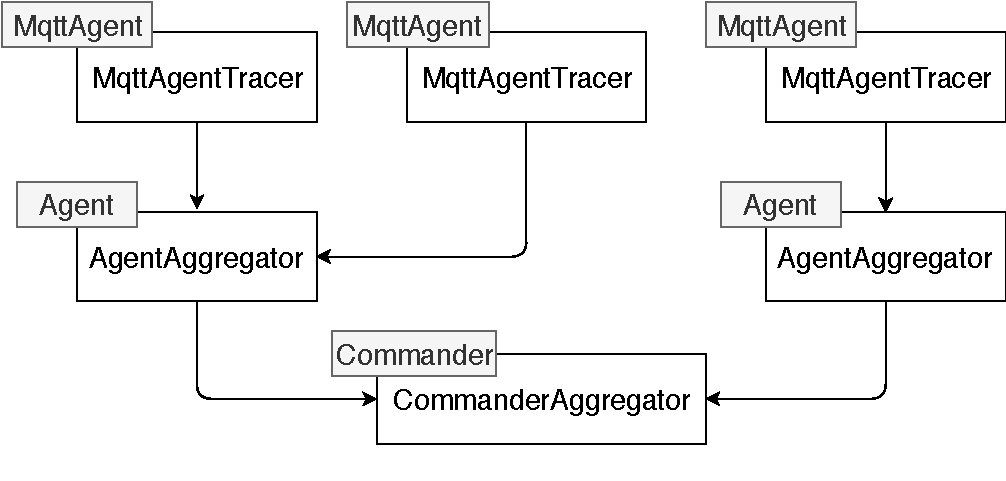
\includegraphics[scale=0.75]{Resources/PDF/ReportingArchitecture}
		\caption{Reporting Architecture}
		\label{fig:ReportingArchitecture}
	\end{center}
\end{figure}
The reporting architecture is organized in strong accordance to Varroas hierarchy.
The data flow of the report happens bottom up from the Agents to the Commander.
The reported data is recorded at the lowest level of the hierarchy namely the \emph{MqttAgentTracer} which tracks its MQTT Agents Actions.
Subsequently the \emph{AgentAggregator} receives this data and aggregates it before passing the result to the Commander.
The Commander aggregator collects the received data and then aggregates the information of all Agents and compiles it into the report.
Figure \ref{fig:ReportingArchitecture} visualizes the relationships between the components explained above.

\section{Metrics}
\subsection{Duration Sampler}
The duration Sampler gives metrics based on the duration of the executed Actions:
\begin{itemize}
	\item \textbf{count:} the amount of executed Actions.
	\item \textbf{mean:} the mean duration of the executed Actions.
	\item \textbf{stdDev:} the standard deviation of the duration of the executed Actions.
	\item \textbf{min:} the minimum duration of the executed Actions.
	\item \textbf{max:} the maximum duration of the executed Actions.
\end{itemize}
\subsection{Lateness Sampler}
The Duration Sampler reports metrics based on the lateness of expected durations of the executed Actions:
\begin{itemize}
	\item \textbf{count:} the amount of Actions whose durations exceeded the expected duration.
	\item \textbf{mean:} the mean lateness value of the actions.
	\item \textbf{stdDev:} the standard deviation of the executed Actions lateness.
	\item \textbf{min:} the minimum lateness of the executed Actions.
	\item \textbf{max:} the maximum lateness of the executed Actions.
\end{itemize}

\subsection{Failed Count}
The failed count indicates how many of the Actions were executed unsuccessfully.




\chapter{Requirements}
The following sections list the requirements and their respective priorities.
Additionally it is indicated whether and how they are currently implemented.

\section{Non-Functional Requirements}

\paragraph{Transparency (Must Have High)}\label{sec:Transparency}
\emph{Varroa has to be comprehensible for the user.}

This requirement is fulfilled.
Varroa implements expressive logging with configurable levels and outputs.
This enables a rich insight in the execution process of a Varroa test.

\paragraph{10.000.000 MQTT Clients (Must Have High)} 
\emph{Varroa has to be able to generate a large amount of clients.}

The fulfilment of this requirement is not verified yet.

\paragraph{Scalability (Must Have)} 
\emph{Varroa should scale vertically with relatively low scaling costs.}

This requirement is fulfilled.
To do so Varroa is organised as a distributed System and can easily be extended with new instances running as Agents.

\paragraph{Determinism (Must Have)} 
\emph{Varroa has to work in deterministic ways, meaning it should produce the same result for the same Scenario every time.}

This requirement is fulfilled.
To guarantee this determinism several measures are taken, ensuring deterministic distribution and execution of a Scenario (see chapter \ref{sec:Architecture}).

\paragraph{Distributed (Must Have Low)} 
\emph{Varroa is a distributed System.}

This requirement is fulfilled.
Varroa is organized as a distributed System.
It is composed of a Commander and multiple Agents.
These components can be run on separate machines. 
 
\paragraph{Usabillity (Very Important)} 
\emph{Varroa has to be easily usable.}

This requirement is fulfilled.
The user can easily define custom Scenarios as XML files and execute them (see chapter \ref{sec:ScenarioConcept} and \ref{sec:Execution}).

\paragraph{Code Quality (Important)} 
\emph{Varroa's code quality should be very high.}

This requirement is fulfilled.
To ensure high code quality several measures are taken.
An example for these measures is the consequent use of nullability as well as broad test code coverage. 
Also before new code could be added to the master branch it was reviewed by another team member.

\paragraph{Stability (Important)} 
\emph{Varroa has to run in a stable manner.}

This requirement is fulfilled.
Stability is ensured by the use of integration tests and general unit tests.

\paragraph{Resource efficiency (Important)} 
\emph{Varroa has to use the available computation and memory resources efficiently.}
%TODO how was this verified.

\paragraph{User / Developer Guide (Somewhat Important)} 
\emph{Varroa needs a User / Developer Guide.}

This requirement is fulfilled.
The documentation educates the user on the definition of a custom scenario as well as the execution of it on his Varroa Distributed System (\ref{sec:ScenarioConcept} and \ref{sec:Execution}).

\paragraph{Automation capacity (Somewhat Important)} 
\emph{Varroa should be automatable.}

%TODO Docker.
%TODO is this fulfilled? 

\paragraph{User Interface}
\emph{Varroa should have a well designed user interface with high usability.}

This requirement is fulfilled.
The user can interact with Varroa using a command line interface.

\paragraph{Multi Platform Support (Nice To Have)}
\emph{Varroa should run on multiple platforms.}

This requirement is fulfilled.
Due to the utilisation of Docker, Varroa can run on several platforms (see chapter \ref{sec:Execution}).

\section{Functional Requirements}
The following sections list the non-functional requirements and their respective priorities.

\paragraph{Scenarios (Must Have High)}
\emph{Varroa must be able to execute user defined MQTT Scenarios.}

This requirement is fulfilled.
Varroa has the ability to parse and execute Scenarios, according to the concept explained in chapter \ref{sec:ScenarioConcept}.

\paragraph{MQTT Specification Confirmity (Must Have High)}
\emph{Varroa must conform to the MQTT specification.}

This requirement is fulfilled.
Varroa uses the HiveMQ MQTT Client library for its MQTT Actions.
The library ensures specification conformity in both MQTT version 3 and MQTT version 5.

\paragraph{All Transports (Must Have)}
\emph{Varroa has to support all transports that are possible in MQTT.}

This requirement is not fulfilled.
Currently Varroa does not support websockets.

\paragraph{Reports (Must Have)}
\emph{Varroa has to report the findings of the testing process.}

This requirement is fulfilled.
Varroa supports reporting findings of tests (see \ref{sec:Reporting})

\paragraph{User Feedback (Must Have Low)}
\emph{Varroa has to give user feedback during runtime.}

This requirement is fulfilled (see \ref{sec:Transparency}).

\paragraph{Documentation (Very Important)}
\emph{Varroa has to be documented. }

This requirement is fulfilled.
This document contains a user guide and briefly explains the architecture and inner workings of Varroa.

\paragraph{Metrics (Very Important)}
\emph{Varroa has to record and expose internal metrics.}

This requirement is not fulfilled.

\paragraph{Deployment Convenience (Important)}
\emph{Varroa must be easily deployable.}

This requirement is fulfilled. Due to the use of Docker Varroa Instances can be easily started and so a Varroa Distributed System can be orchestrated without much configuration (see chapter \ref{sec:Execution}).

\paragraph{Topology Change (Less important)}
\emph{Varroa must be able to simulate changes to the network topology.}

This requirement is not fulfilled.
It is not possible to simulate network level behaviour of the clients in the current version.

\paragraph{Simple and Expert Mode (Somewhat Important}
\emph{Varroa has to have two user modes.
One for experienced users and one for unexperienced users.}

This requirement is not fulfilled.
Since Varroa does not have a graphical user interface in this version.
Simple and Expert modes are not implemented.


\paragraph{Notifications (Nice To Have)}
\emph{Varroa must notitfy the user about the testing process by Email.}

This requirement is not fulfilled in the current version.

% Abbildungsverzeichnis generieren.
\clearpage
\addcontentsline{toc}{chapter}{\listfigurename}
\listoffigures

% Tabellenverzeichnis generieren.
%\clearpage
%\addcontentsline{toc}{chapter}{\listtablename}
%\listoftables

% Listingverzeichnis generieren.
\clearpage
%\renewcommand{\lstlistlistingname}{Listingverzeichnis}
\addcontentsline{toc}{chapter}{\lstlistlistingname}
\lstlistoflistings

\end{document}
